\documentclass[supercite]{Experimental_Report}

\title{机器学习算法实现}
\course{计算机科学与技术学院}
\author{xxx}
\school{x年x月x日}
\classnum{CS23xx}
\stunum{U2023xxxx}
\instructor{} % 李平、孙伟平、范晔斌、陈加忠

\usepackage{tikz}
\usetikzlibrary{mindmap,trees}%包含了 TikZ 库,用于在文档中绘制图形。
\usepackage{algorithm, multirow}
\usepackage{algpseudocode}%包含了算法环境,用于在文档中编写算法。
\usepackage{amsmath}
\usepackage{amsthm}%包含了数学符号和环境,用于在文档中编写数学公式。
\usepackage{framed}
\usepackage{fontspec}%包含了使用非 TeX 字体的功能
\setmainfont{FandolSong}
\setsansfont{FandolSong}
\usepackage{mathtools}%包含了高级数学符号和工具
\usepackage{subcaption}%包含了子图环境,用于在文档中创建多个子图
\usepackage{amsmath, amssymb, amsfonts}
%\usepackage{tabu}
\usepackage{xltxtra} %提供了针对XeTeX的改进并且加入了XeTeX的LOGO, 自动调用xunicode宏包(提供Unicode字符宏)
\usepackage{bm}%包含了粗体字符的功能
\usepackage{longtable}%包含了长表格环境
\usepackage{tikz}
\usepackage{tikzscale}
\usepackage{pgfplots}%包含了画图的功能
%\usepackage{enumerate}
\usepackage{graphicx}%包含了图像插入功能
\pgfplotsset{compat=1.16}

\newcommand{\cfig}[3]{
  \begin{figure}[htb]
    \centering
    \includegraphics[width=#2\textwidth]{images/#1.tikz}
    \caption{#3}
    \label{fig:#1}
  \end{figure}
}

\newcommand{\sfig}[3]{
  \begin{subfigure}[b]{#2\textwidth}
    \includegraphics[width=\textwidth]{images/#1.tikz}
    \caption{#3}
    \label{fig:#1}
  \end{subfigure}
}

\newcommand{\xfig}[3]{
  \begin{figure}[htb]
    \centering
    #3
    \caption{#2}
    \label{fig:#1}
  \end{figure}
}
%上述定义了用于在文档中插入图片的命令
\newcommand{\rfig}[1]{\autoref{fig:#1}}
\newcommand{\ralg}[1]{\autoref{alg:#1}}
\newcommand{\rthm}[1]{\autoref{thm:#1}}
\newcommand{\rlem}[1]{\autoref{lem:#1}}
\newcommand{\reqn}[1]{\autoref{eqn:#1}}
\newcommand{\rtbl}[1]{\autoref{tbl:#1}}

\algnewcommand\Null{\textsc{null }}%定义了一个新的命令 \Null,用于在算法中插入 null 的格式化文本。
\algnewcommand\algorithmicinput{\textbf{Input:}}%用于更改算法中输入部分的默认格式。
\algnewcommand\Input{\item[\algorithmicinput]}
\algnewcommand\algorithmicoutput{\textbf{Output:}}
\algnewcommand\Output{\item[\algorithmicoutput]}
\algnewcommand\algorithmicbreak{\textbf{break}}
\algnewcommand\Break{\algorithmicbreak}
\algnewcommand\algorithmiccontinue{\textbf{continue}}
\algnewcommand\Continue{\algorithmiccontinue}
\algnewcommand{\LeftCom}[1]{\State $\triangleright$ #1}
%上述代码定义了一些新的命令,用于在编写算法时更改默认的算法环境。使用这些命令可以使算法更加美观和易读。

\newtheorem{thm}{定理}[section]
\newtheorem{lem}{引理}[section]

\colorlet{shadecolor}{black!15}%定义了一个名为 shadecolor 的颜色变量,并将其设置为黑色的 15% 不透明度。

\theoremstyle{definition}
\newtheorem{alg}{算法}[section]
\def\thmautorefname~#1\null{定理~#1~\null}
\def\lemautorefname~#1\null{引理~#1~\null}
\def\algautorefname~#1\null{算法~#1~\null}
\usepackage{xcolor}
\usepackage{listings}
\usepackage[skins]{tcolorbox}
\tcbuselibrary{breakable}
%下述代码定义了一个新的环境,叫做 abox,它是基于 tcolorbox 包中的 tcolorbox 环境构建的。
\newtcolorbox{abox}[1][]{enhanced,
	fonttitle = \heiti \large \bfseries,% 标题字体设置
	colbacktitle =black,% 标题背景颜色
	coltitle=white,% 标题字体颜色
	% halign title=center,% 标题对齐方式
	attach boxed title to top left = {yshift = -5pt},
	%	将标题以box 形式放在文本框左上角,并向下移动5pt	
	%----------正文字体--------
	fontupper = \kaishu,%正文字体设置
	%colback = white,%正文背景颜色设置
	%---------边框设置---------
	arc = 4pt,%正文边框边角弧度
	%	boxed title style={arc=0pt},%标题框边角弧度
	colframe=black,%边框颜色设置
	toprule  = 1pt,%取消上边框
	rightrule = 1pt,%取消下边框
	%---------调整字体位置------
	top = 10pt,%增大正文文本与上边框距离
	%---------设置标题为默认参数,不影响其他参数的设置
	title=#1,
	breakable
}
%abox 环境是一个可以换行的带标题的文本盒子。比如, 你可以用 \begin{abox}[标题] 和 \end{abox} 来把一段文本放在这个环境里面, 并且会自动加上标题和格式.
\newcommand{\tabincell}[2]{\begin{tabular}{@{}#1@{}}#2\end{tabular}}  

\begin{document}

\maketitle
\clearpage
\pagenumbering{Roman}
\tableofcontents[level=2]
\clearpage
\pagenumbering{arabic}

\section{线性回归}
\subsection{什么是线性回归}
就是通过一系列输入和对应的输出,建立输出与输入的一次关系,再通过模型进行预测

\subsection{线性回归的目的}
根据以往的数据训练模型,预测新样本的输出
\subsection{输入输出}
输入为$$x_1^1,x_1^2,\cdot\cdot,x_2^1,x_2^2,\cdot\cdot\cdot,x_i^1,x_i^2\cdot\cdot,x_i^k$$

输出为$$y_1,y_2,\cdot\cdot\cdot,y_i$$
\subsection{模型的数学描述}
(1)\texttt{单变量:$$y_i=w\cdot x_i+b$$}

(2)\texttt{多变量:$$y_i=w_1\cdot x_i^1+w_2\cdot x_i^2+\cdot\cdot\cdot+w_k\cdot x_i^k$$}
\subsection{模型训练流程}
(1)\texttt{单变量:最小二乘法,运用求偏导为0最小化均方误差MSE}

$$
(w^*, b^*) =\underset{(w, b)}{\arg \min } \sum_{i=1}^{m}\left(f(x_{i})-y_{i}\right)^2 \\ 
=\underset{(w, b)}{\arg \min } \sum_{i=1}^m(y_i-w x_i-b)^2 

$$

推导得到
$$
 w=\frac{\displaystyle \sum_{i=1}^m y_i(x_i-\overline{x})}{ \displaystyle \sum_{i=1}^m x_i^2-\frac{1}{m}(\sum_{i=1}^{m} x_{i})^{2}} \\
 $$
 $$
b=\frac{1}{m} \sum_{i=1}^m (y_i-w x_i)
$$

(2)\texttt{多变量:一个输出$y_i$由k个属性决定$\{(x_1,x_2,\cdots,x_k)\}$
我们习惯使用矩阵形式:
$$Y=X * \hat{w}=x^T*w+b $$
$$\hat{w}=(w ; b)=\left(\begin{array}{c}w_1 \\ w_2 \\ {\cdots} \\ w_k \\ b \end{array}\right) 
$$
$$
X=\left(\begin{array}{ccccc} 
x_{11} & x_{12} & \dots & x_{1k} & 1 \\ 
x_{21} & x_{22} & \dots & x_{2k} & 1 \\ 
\vdots & \vdots & \ddots & \vdots & \vdots \\ 
x_{i1} & x_{i2} & \dots & x_{ik} & 1 
\end{array}\right)
$$
$$
X * \hat{w} &=\left(\begin{array}{ccccc} 
x_{11} & x_{12} & \dots & x_{1k} & 1 \\ 
x_{21} & x_{22} & \dots & x_{2k} & 1 \\ 
\vdots & \vdots & \ddots & \vdots & \vdots \\ 
x_{i1} & x_{i2} & \dots & x_{ik} & 1 
\end{array}\right) * 
\left(\begin{array}{c} w_1 \\ w_2 \\ \dots \\ w_k \\ b \end{array}\right)\\
=\left(\begin{array}{c}
w_1 x_{11} + w_2 x_{12} + \ldots + w_d x_{1k} + b \\ 
w_1 x_{21} + w_2 x_{22} + \ldots + w_d x_{2k} + b \\ 
\cdots \\ 
w_1 x_{i1} + w_2 x_{i2} + \ldots + w_d x_{ik} + b 
\end{array}\right)\\
$$
}

“广义的线性模型”(generalized linear model),其中,$g(\cdot)$称为联系函数(link function)。
$$y=g^{-1}(w^T x + b)$$

\subsection{偏差与方差}
偏差指的是预测的期望值与真实值的偏差,方差则是每一次预测值与预测值的期望之间的差均方

偏差体现了学习器预测的准确度,刻画学习器的拟合能力,而方差体现了学习器预测的稳定性

偏差-方差窘境(bias-variance dilamma):随着训练程度的提升,偏差越来越小(预测值与真实值之间的差异越来越小);方差值越来越大(学习算法对数据集的波动越来越敏感)

所以训练次数不是越多越好,适度而止
\subsection{梯度下降训练法}



(1)单变量最小二乘,求偏导=0
$$
E_{(w, b)}=\sum_{i=1}^{m}(y_{i}-w x_{i}-b)^2 \\
$$

$$
\frac{\partial E_{(w, b)}}{\partial w} =2\left(w \sum_{i=1}^m x_i^2-\sum_{i=1}^m (y_i-b) x_{i}\right) = 0 \\ 
$$
$$
\frac{\partial E_{(w, b)}}{\partial b} =2\left(m b-\sum_{i=1}^m (y_i-w x_i) \right) = 0 \\
$$

(2)多变量:
令$E_{\hat{w}}=(y-X\hat{w})^T (y-X\hat{w})$,对$\hat{w}$求导可得:  

$\displaystyle \therefore \frac{\partial E_{\hat{w}}}{\partial \hat{w}}=2 X^T(X \hat{w}-y) = 0$  

$\therefore \hat{w}^*=(X^T X )^{-1} X^T y, f(\hat{x}_i)=\hat{x}_i^T(X^T X)^{-1} X^T y$  

\begin{figure}[ht]
\centering
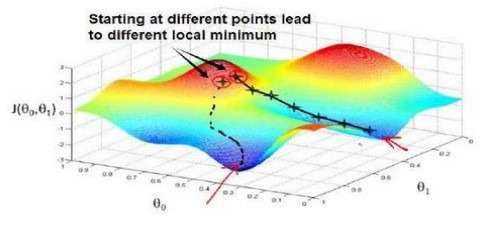
\includegraphics[scale=1.0]{image/gradient_descent.jpg}
\caption{梯度下降}
\label{fig:p1}
\end{figure}


\subsection{过拟合与欠拟合}
学习能力过强,以至于把训练样本所包含的不太一般的特性都学到了,称为:过拟合(overfitting)

学习能太差,训练样本的一般性质尚未学好,称为:欠拟合(underfitting)。

我们希望得到的是在新样本上表现得很好的学习器,即泛化误差小,普适性强。
\subsection{算法代码}

\begin{algorithm}[htb]
\caption{线性回归}
\label{alg:F4}
\hspace*{0.02in} {\bf Input:}
数据集,包含$(x_1,x_2...x_i)$与$y_1,y_2...y_i$

\hspace*{0.02in} {\bf Output:} 模型预测率
  \begin{algorithmic}[1]
    \State
        数据清洗:包括划分数据集交叉验证、划分X与Y
    \State
        计算代价函数:代价函数为均方误差
    \State
        设置学习率与迭代次数,梯度下降:
        $$ \theta_j:= \theta_j-α\frac{\mathrm{d}}{\mathrm{d}\theta_j}J(\theta_0,\theta_1) 
        $$这里$\theta_0$相当于w,$\theta_1$相当于b
    \State
        结合测试集求预测率
  \end{algorithmic}
\end{algorithm}
\clearpage

\section{逻辑回归}
\subsection{和线性回归的区别和联系}
(1)区别:逻辑回归不是通过模型预测值,而是尝试预测的结果是否属于一个类别(答案表现为正确或者错误)适用于标签y为离散化的情形。
比如:判断一封电子邮件是否是垃圾邮件;判断一次金融交易是否是欺诈,区别一个肿瘤是恶性的还是良性的。

(2)联系:逻辑回归之所以还是回归因为采用线性模型实现分类任务。

\subsection{逻辑回归的训练流程}
(1)为了实现分类问题,我们建立一个逻辑回归模型:$h_\theta(x)=g(\theta^TX)$
其中: $X$代表特征向量,$g$代表逻辑函数,常用的逻辑函数为 S 形函数sigmoid :
$$g(z)=\frac{1}{1+e^{-z}}$$
当$h_\theta(x)$>=0.5,预测y=1
当$h_\theta(x)$<0.5时,预测y=0

(2)线性回归中代价函数是所有模型误差的平方和,但是当代入$g(z)$这样的逻辑函数后体现为多个局部最小值,影响全局最小值的计算
逻辑回归中的代价函数:
$$\operatorname{Cost}\left(h_{\theta}(x), y\right)=-y \times \log \left(h_{\theta}(x)\right)-(1-y) \times \log \left(1-h_{\theta}(x)\right)
$$
拓展到代价函数为:
$$
J(\theta)=\frac{1}{m} \sum_{i=1}^{m}\left[-y^{(i)} \log \left(h_{\theta}\left(x^{(i)}\right)\right)-\left(1-y^{(i)}\right) \log \left(1-h_{\theta}\left(x^{(i)}\right)\right)\right] \mid
$$

$$
即:  J(\theta)=-\frac{1}{m} \sum_{i=1}^{m}\left[y^{(i)} \log \left(h_{\theta}\left(x^{(i)}\right)\right)+\left(1-y^{(i)}\right) \log \left(1-h_{\theta}\left(x^{(i)}\right)\right)\right] 
$$

(3)在得到这样一个代价函数以后,我们便可以用梯度下降算法来求得能使代价函数最小的参数了。
 $$ \theta_j:= \theta_j-α\frac{\mathrm{d}}{\mathrm{d}\theta_j}J(\theta) 
$$

\clearpage
\subsection{算法代码}
\begin{algorithm}[htb]
\caption{逻辑回归}
\label{alg:F4}
\hspace*{0.02in} {\bf Input:}
数据集,包含$(x_1,x_2...x_i)$与$y_1,y_2...y_i$

\hspace*{0.02in} {\bf Output:} 模型预测率
  \begin{algorithmic}[1]
    \State
        数据清洗:包括划分数据集交叉验证、划分X与Y、正则化(调节参数大小)、特征缩放
    \State
        求出逻辑函数$g(z)=\frac{1}{1+e^{-z}}$
        并计算$h_\theta(x)=g(\theta^TX)$
    \State
        计算代价函数:代价函数为逻辑回归的$Cost(h_\theta(x),y)$和对应的$J(\theta)$
    \State
        设置学习率与迭代次数,梯度下降:
        $$ \theta_j:= \theta_j-α\frac{\mathrm{d}}{\mathrm{d}\theta_j}J(\theta) 
        $$
    \State
        结合测试集求预测率
  \end{algorithmic}
\end{algorithm}
\clearpage
\section{支持向量机}
\subsection{SVM的由来}
Support Vector Machine (SVM) 是一种监督学习模型,它的目标是在二类和多类分类问题中找到最优超平面。 SVM是基于结构风险最小化原理,它的基本思想是对于给定的训练数据集,通过找到最优超平面将其划分为两个类别,并使得这两个类别之间的间隔最大。
\subsection{SVM的迭代过程}
(1)首先,对于给定的训练数据集,通过特征映射将其映射到高维空间中。

(2)然后,在高维空间中寻找一个最优超平面,使得两类数据间的间隔最大。这个过程通常是通过求解凸二次规划问题来实现的。

(3)接着,根据找到的最优超平面对训练数据进行分类,并计算分类误差。

(4)如果分类误差过大,则需要对模型进行修正,通过调整模型参数或者选择新的特征来减小误差。

(5)重复上述步骤直到模型误差达到最小或者达到最大迭代次数。在实际使用中,我们还可以通过设置终止条件来控制迭代过程,比如设置最小误差阈值或者最小迭代步长。当算法达到这些条件时,就可以停止迭代,以保证算法的效率。

\subsection{SVM的核函数}
SVM 算法通过核函数将数据映射到高维空间中,以找到一个最优超平面。
核函数是一种特殊的函数,能够将线性不可分的数据转化成线性可分的数据,从而解决线性模型无法解决的问题。

例如:假设我们有一个二维数据集,其中一部分数据是圆形的,另一部分数据是线性的,我们使用线性SVM模型对其进行分类。显然,在二维空间中是无法找到一条直线将两类数据完全分开的。
如果我们使用高斯核函数将数据映射到高维空间中,由于高斯核函数能够将圆形的数据转换为线性的数据,因此我们就能在高维空间中找到一个超平面将两类数据完全分开。

它对于给定的输入 x 和 y,返回一个核矩阵 K(x, y)。核矩阵 K(x, y) 的元素 K($x_i$, $x_j$) 表示 $x_i$ 和 $x_j$ 在高维空间中的点积。

常见的核函数有:
(1)\texttt{线性核函数:$K(x,y) = x * y$}

(2)\texttt{高斯核函数:$K(x,y)=e\left(-\frac{\left\|x-l^{(1)}\right\|^{2}}{2 \sigma^{2}}\right)$}

(3)\texttt{多项式核函数:$K(x,y)=(x*y+r)^d$}

(4)\texttt{sigmoid核函数:$K(x,y)=\tanh{kx * y + r}$}
\subsection{算法代码}
\begin{algorithm}[htb]
\caption{SVM}
\label{alg:F4}
\hspace*{0.02in} {\bf Input:}
数据集,包含$(x_1,x_2...x_i)$与$y_1,y_2...y_i$的数据集

\hspace*{0.02in} {\bf Output:} 模型预测率
  \begin{algorithmic}[1]
    \State
        数据清洗:包括划分数据集交叉验证、划分X与Y,调参,特征选择
    \State
        创建 SVM 分类器,使用线性核
    \State
        训练模型
    \State
        结合测试集求预测率
  \end{algorithmic}
\end{algorithm}
\clearpage
\section{k-means算法}
\subsection{什么叫聚类}
聚类算法是一种无监督学习算法,它的目的是将数据集中的样本分为若干组,每组样本被称为一个簇。聚类算法通过找出数据集中相似样本之间的关系,将样本分为不同的簇。
\subsection{聚类的目的}
聚类算法的目的是将数据集中的样本分为若干组,每组样本被称为一个簇。通过对数据进行聚类,可以实现:

(1)发现数据集中隐藏的模式:聚类算法能够将数据集中相似的样本分到同一簇中,这样就能发现数据集中隐藏的模式。

(2)简化并压缩数据:聚类算法能够将数据简化成若干簇,这样就能够更容易地理解数据,缩成若干个簇,这样就能够减少数据存储和运算的复杂度。

(3)数据分类:聚类算法能够将数据分为几类,这样就能够为后续的分析和决策提供便利。

(4)发现异常值:聚类算法能够将数据分类,如果有些样本不属于任何簇,就可能是异常值。

\subsection{聚类的输入输出}
(1)输入:始数据集,这个数据集可能包含多维特征和样本标签。输入数据集的格式可能是矩阵或者数组形式。

(2)输出:聚类结果,这个结果可能包括聚类中心、每个样本所属的簇、聚类的质量度量值等。输出结果的格式可能是矩阵或者数组形式,也可能是图形化展示。
\subsection{无监督和有监督算法的区别}
非监督学习算法。我们将要让计算机学习无标签数据,而不是此前的标签数据。
在一个典型的监督学习中,我们有一个有标签的训练集,我们的目标是找到能够区分正样本和负样本的决策边界,在这里的监督学习中,我们有一系列标签,我们需要据此拟合一个假设函数。
不同的是,在非监督学习中,我们的数据没有附带任何标签,仅是一些数据集
\subsection{算法代码}
K-均值最小化问题,是要最小化所有的数据点与其所关联的聚类中心点之间的距离之和
$$
J\left(c^{(1)}, \ldots, c^{(m)}, \mu_{1}, \ldots, \mu_{K}\right)=\frac{1}{m} \sum_{i=1}^{m}\left\|X^{(i)}-\mu_{c^{(i)}}\right\|^{2}
$$

$
其中  \mu_{c^{(i)}}  代表与  x^{(i)}  最近的聚类中心点。
$

$
我们的的优化目标便是找出使得代价函数最小 的  c^{(1)}, c^{(2)}, \ldots, c^{(m)} 
和  \mu^{1}, \mu^{2}, \ldots, \mu^{k}  
$
\begin{algorithm}[htb]
\caption{K-means}
\label{alg:F4}
\hspace*{0.02in} {\bf Input:}
数据集,包含$(x_1,x_2...x_i)$没有标签,想要分类的中心数k

\hspace*{0.02in} {\bf Output:} 聚类划分后的模型
  \begin{algorithmic}[1]
    \State
        读取数据集,不含标签,并对K个中心随机初始化
    \State
        *遍历测试集把每个$X_i$分配给最近的中心
    \State
        *按照第一步的分配将中心移动到所有点的均值位置
    \State
        *循环上面两步,直到达到迭代次数或者中心不再变化
    \State
        战术聚类结果或者输出簇中心的坐标
  \end{algorithmic}
\end{algorithm}
\clearpage

\end{document}
